\subsection{Part 3: Photocurrent delay}

\begin{figure}
    \centering
    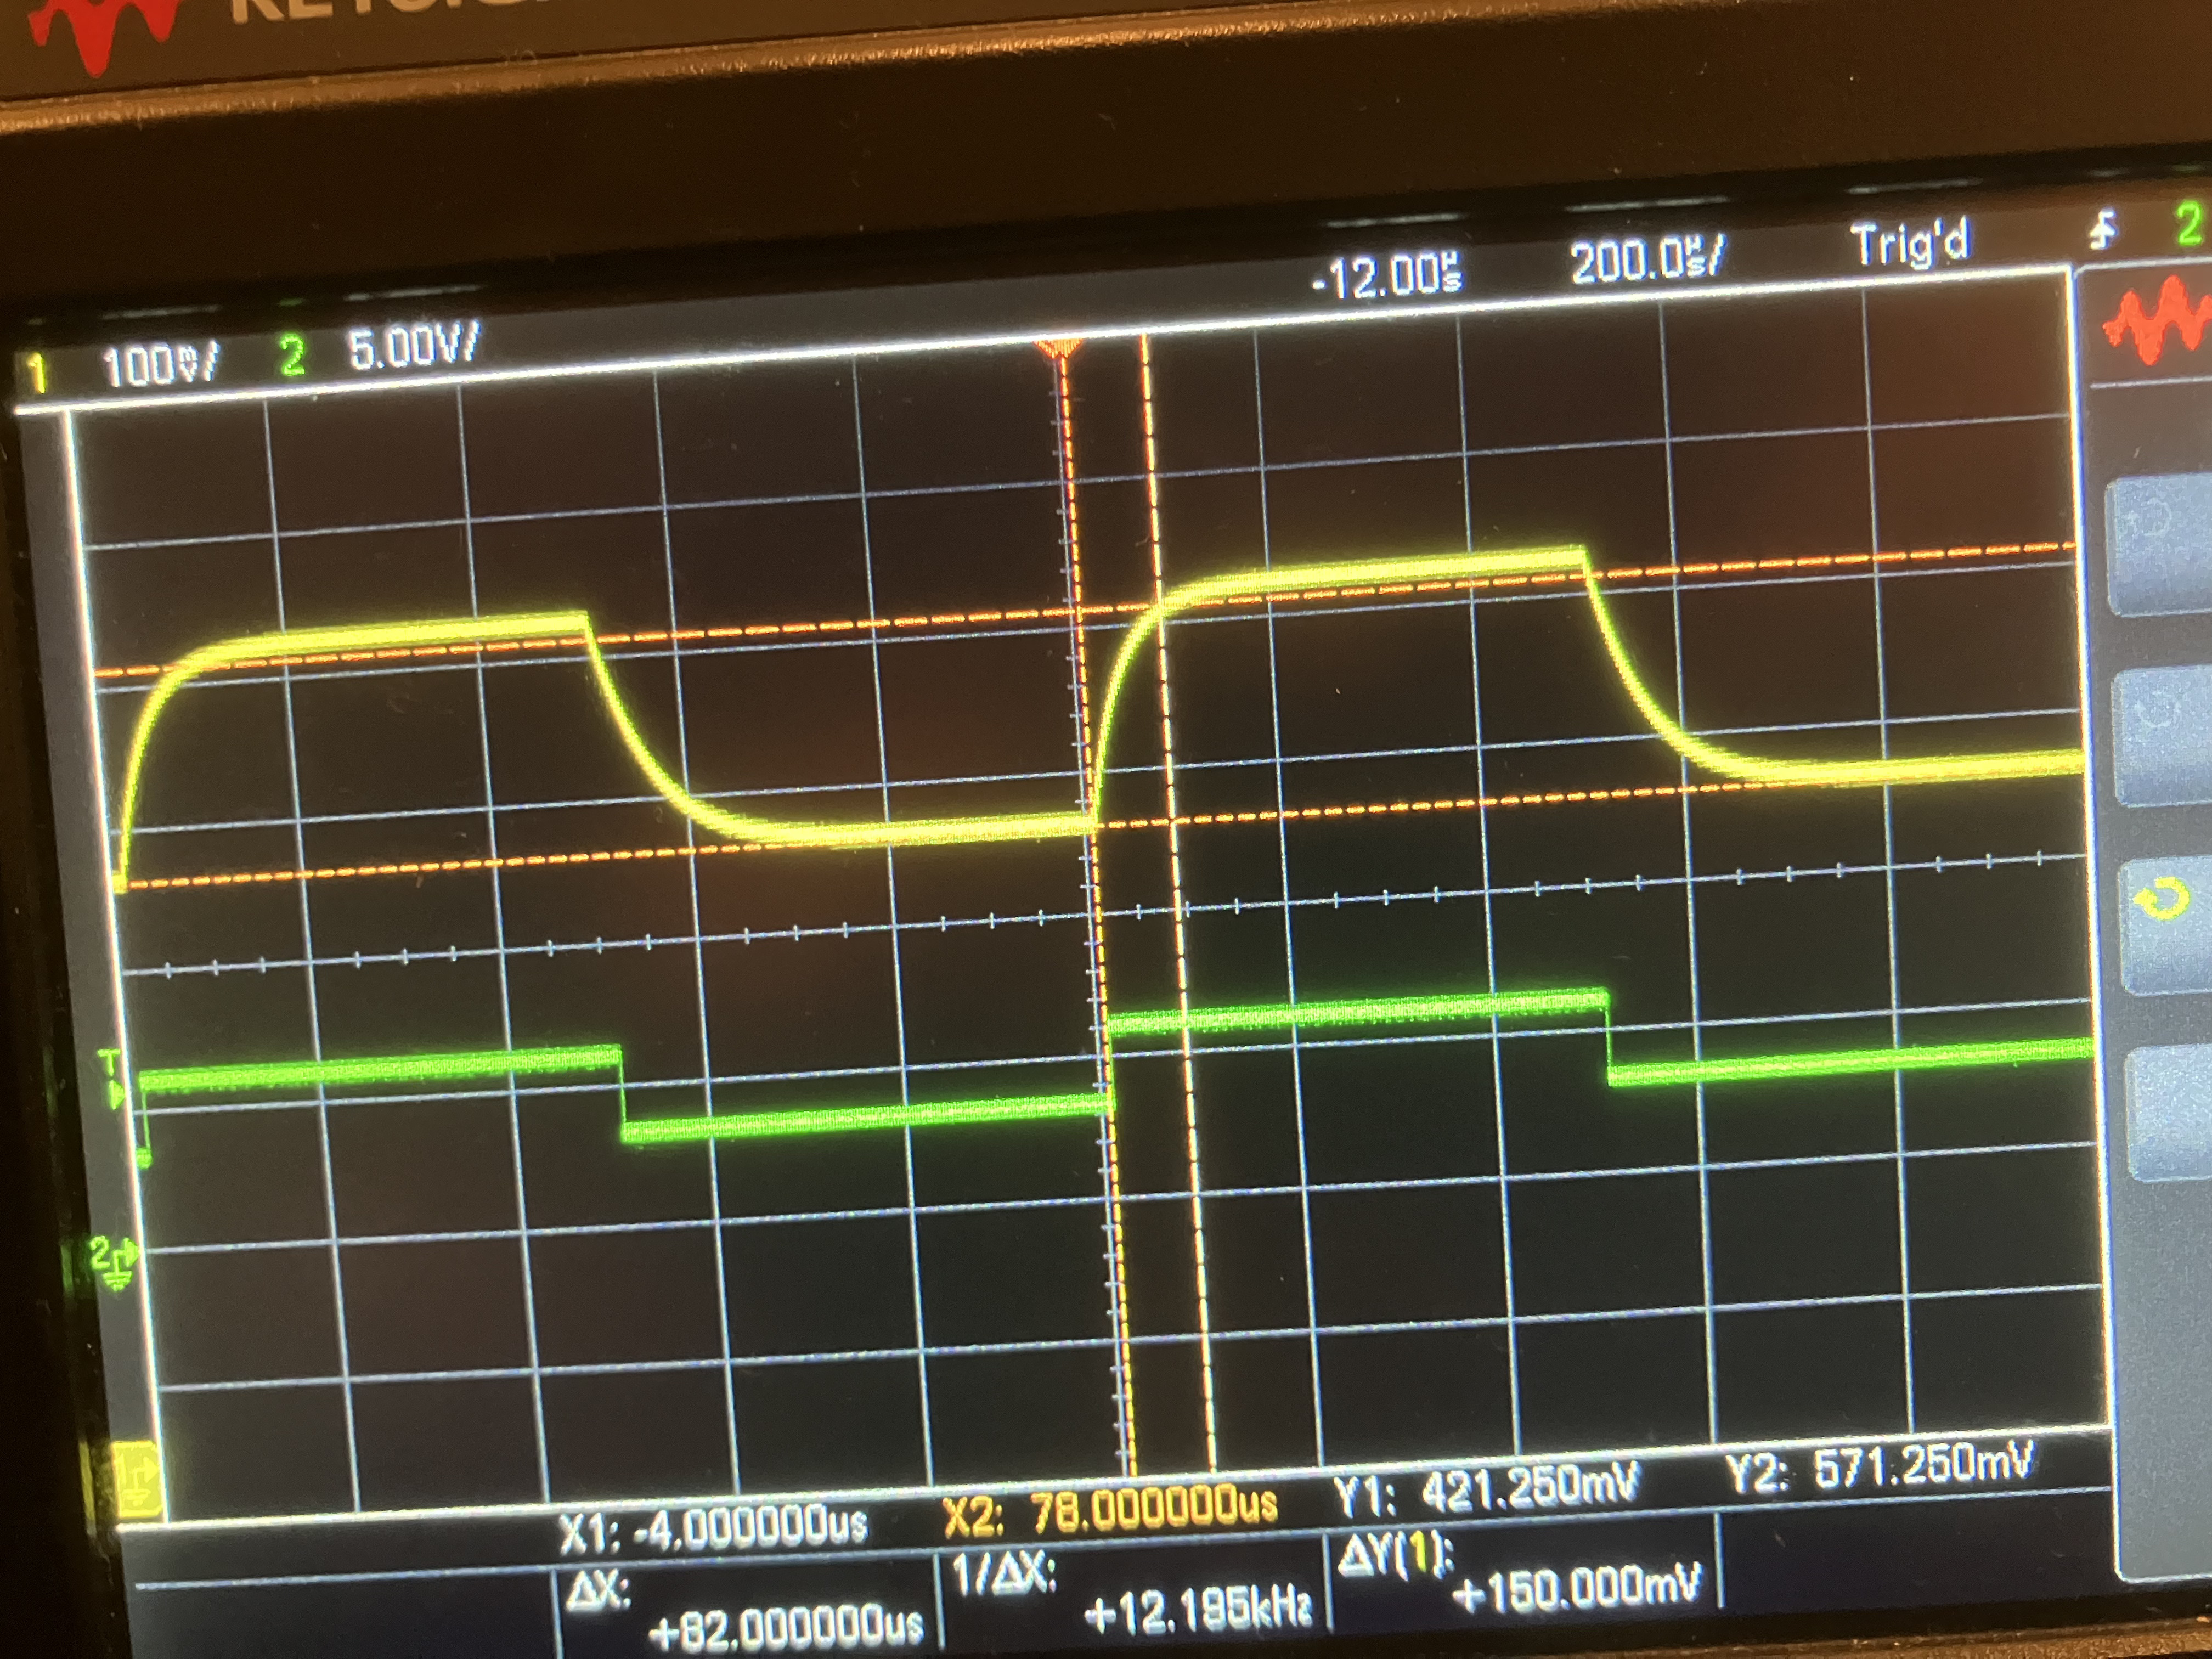
\includegraphics[width=0.8\textwidth]{Results/Part3/V_Func.jpg}
    \caption{Transient Voltage Response of the Phototube}
    \label{fig:V_Func}
\end{figure}

The transient response of the phototube is shown in Figure \ref{fig:V_Func}. The minimum voltage was measured at $(421.250 \pm 0.250)~[mV]$, and the maximum voltage at $(578.750 \pm 0.250)~[mV]$, where the uncertainty comes from the resolution of the cursors in the oscilloscope. Thus, the $95\%$ voltage was at $421.25 + (578.750-421.250) \cdot 0.95 = (570.88 \pm 0.24)~[mV]$, and it took $(78.0 \pm 1.0) - (-4.0 \pm 1.0) = (82.0 \pm 1.4)~[\mu s]$ to reach this voltage. Thus, since the response follows an exponential decay, the time constant can be calculated as:
\begin{gather*}
    \tau = \frac{(82 \pm 1.4)~[\mu s]}{-ln(0.05)} = (27.4 \pm 0.5)~[\mu s]
\end{gather*}

Then, we can find the average power of each electron using Equation \textbf{EDIT}:
\begin{gather*}
    P_e = 60\pm1~[mW] \frac{(0.3 \pm 0.1~[nm])^2}{3.23\pm 0.01~[cm^2]} = (1.7 \pm 1.1) \times 10^{-17}~[W] = 104 \pm 70~[eV/s]
\end{gather*}

Thus, using the Work Function from Equation \ref{eq:work_function}, we can calculate the time for the electron to absorb the required energy to release:
\begin{gather*}
    t = \frac{1.33 \pm 0.07~[eV]}{104 \pm 70~[eV/s]} = (0.013 \pm 0.009)~[s] = (13 \pm 9)~[ms]
\end{gather*}

This is significantly longer than the experimentally-derived time constant, which suggests that the electrons do not absorb energy in a continuous process, instead getting energy in packets, or quanta, as hypothesized by Einstein.